\documentclass[10pt,a4paper]{article}
\usepackage[a4paper,top=3.3cm,bottom=2.1cm,left=1.5cm,right=1.5cm,headheight=42pt,headsep=10pt,footskip=24pt]{geometry}
\usepackage[T1]{fontenc}
\usepackage{amsmath,amssymb}
\usepackage{xcolor}
\usepackage{tikz}
\usetikzlibrary{arrows.meta,calc,patterns}
\usepackage{fancyhdr}
\usepackage{lastpage}
\usepackage{tabularx}
\usepackage{array}
\usepackage{multicol}
\usepackage{needspace}
\usepackage{pifont}

\definecolor{spsblue}{RGB}{20,50,120}
\definecolor{spsgrey}{RGB}{110,110,110}
\setlength{\columnsep}{0.8cm}
\setlength{\columnseprule}{0.4pt}

% ---------- header / footer ----------
\pagestyle{fancy}
\fancyhf{}
\renewcommand{\headrulewidth}{0.9pt}
\renewcommand{\footrulewidth}{0.5pt}
\fancyhead[C]{%
  {\Large\bfseries\color{spsblue}SAGAR PUBLIC SCHOOL}\\[2pt]
  {\small\bfseries Integrated Programme \quad$\bullet$\quad Topic: \sheettopic}}
\fancyfoot[L]{\footnotesize Sagar Public School}
\fancyfoot[C]{\footnotesize Integrated Programme \,|\, Gravitation -- Practice Sheet \sheetno}
\fancyfoot[R]{\footnotesize Page \thepage\ of \pageref{LastPage}}
\setlength{\parindent}{0pt}
\setlength{\parskip}{0pt}
\renewcommand{\arraystretch}{1.2}

% ---------- question machinery ----------
\newcounter{qn}
\newcommand{\cursrc}{}
\newenvironment{question}[1]{%
  \par\vspace{6pt}\def\cursrc{#1}%
  \begin{minipage}{\linewidth}\refstepcounter{qn}\textbf{Q.\theqn}\quad\ignorespaces}%
 {\par\vspace{1pt}\hfill{\tiny\color{spsgrey}[\cursrc]}\end{minipage}\par}
\newcommand{\secthead}[1]{\par\vspace{8pt}\noindent\begin{minipage}{\linewidth}{\normalsize\bfseries\color{spsblue}#1}\par\vspace{1pt}\hrule height 0.6pt\end{minipage}\par\nobreak}

\newcommand{\labA}{A}\newcommand{\labB}{B}\newcommand{\labC}{C}\newcommand{\labD}{D}
\newcommand{\numlabels}{\renewcommand{\labA}{1}\renewcommand{\labB}{2}\renewcommand{\labC}{3}\renewcommand{\labD}{4}}
\newcommand{\letterlabels}{\renewcommand{\labA}{A}\renewcommand{\labB}{B}\renewcommand{\labC}{C}\renewcommand{\labD}{D}}
\newcommand{\optsfour}[4]{\par\vspace{2pt}\hspace*{1em}\begin{tabularx}{\dimexpr\linewidth-1em\relax}{*{4}{>{\raggedright\arraybackslash}X}}
 (\labA) #1 & (\labB) #2 & (\labC) #3 & (\labD) #4\end{tabularx}\par}
\newcommand{\optstwo}[4]{\par\vspace{2pt}\hspace*{1em}\begin{tabularx}{\dimexpr\linewidth-1em\relax}{*{2}{>{\raggedright\arraybackslash}X}}
 (\labA) #1 & (\labB) #2 \\ (\labC) #3 & (\labD) #4\end{tabularx}\par}
\newcommand{\optsone}[4]{\par\vspace{2pt}\begin{list}{}{\setlength{\leftmargin}{2.3em}\setlength{\labelwidth}{2em}\setlength{\itemsep}{0pt}\setlength{\topsep}{0pt}\setlength{\parsep}{0pt}}
 \item[(\labA)] #1 \item[(\labB)] #2 \item[(\labC)] #3 \item[(\labD)] #4 \end{list}\par}

\tikzset{fig/.style={line width=0.8pt,>={Stealth[length=2mm]}}}

% Motion Ex-I Q.16 : one square panel / four panels
\newcommand{\sqpanel}[6]{\begin{tikzpicture}[fig,line width=0.7pt]
 \node[left] at (-0.1,0.9) {(#1)};
 \draw (0,0) rectangle (1.8,1.8);
 \foreach \p in {(0.55,1.3),(1.25,1.3),(0.9,0.9),(0.55,0.45),(1.25,0.45)} \fill \p circle (3pt);
 \node[anchor=north west,inner sep=1pt] at (0,1.8) {\scriptsize #2};
 \node[anchor=north east,inner sep=1pt] at (1.8,1.8) {\scriptsize #3};
 \node[anchor=south west,inner sep=1pt] at (0,0) {\scriptsize #4};
 \node[anchor=south east,inner sep=1pt] at (1.8,0) {\scriptsize #5};
 \node[anchor=west,inner sep=2pt] at (0.95,0.92) {\scriptsize #6};
\end{tikzpicture}}
\newcommand{\figSquares}{\sqpanel{A}{5M}{3M}{M}{5M}{M}\hspace{0.5cm}\sqpanel{B}{2M}{3M}{M}{2M}{M}\\[6pt]
 \sqpanel{C}{5M}{3M}{M}{5M}{2M}\hspace{0.5cm}\sqpanel{D}{2M}{3M}{M}{2M}{2M}}

% JEE Main 2026 22 Jan Morning : four masses at corners
\newcommand{\figSquare}{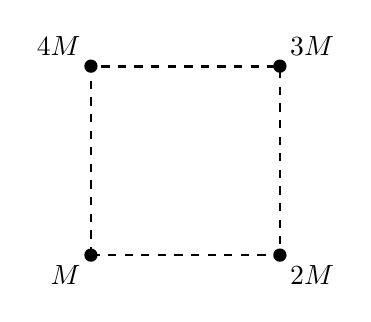
\begin{tikzpicture}[fig]
 \draw[dashed,line width=1pt] (0,0) rectangle (2.4,2.4);
 \foreach \p in {(0,0),(2.4,0),(0,2.4),(2.4,2.4)} \fill \p circle (2.4pt);
 \node[above left] at (0,2.4) {$4M$}; \node[above right] at (2.4,2.4) {$3M$};
 \node[below left] at (0,0) {$M$}; \node[below right] at (2.4,0) {$2M$};
\end{tikzpicture}}

% Motion Ex-I Q.22 : energy versus orbit radius
\newcommand{\figEnergy}{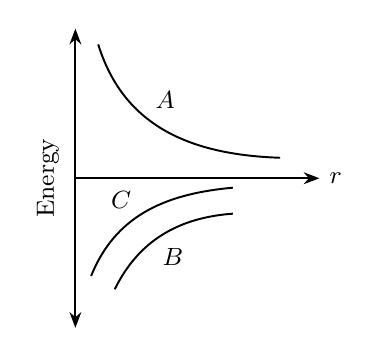
\begin{tikzpicture}[fig,line width=0.7pt]
 \draw[<->] (0,-1.9)--(0,1.9); \node[rotate=90] at (-0.35,0) {\small Energy};
 \draw[->] (0,0)--(3.1,0) node[right] {\small $r$};
 \draw (0.29,1.7) .. controls (0.6,0.7) and (1.4,0.3) .. (2.6,0.26); \node at (1.14,1.0) {\small $A$};
 \draw (0.2,-1.24) .. controls (0.5,-0.5) and (1.1,-0.2) .. (2.0,-0.12); \node at (0.58,-0.28) {\small $C$};
 \draw (0.5,-1.41) .. controls (0.8,-0.8) and (1.3,-0.5) .. (2.0,-0.45); \node at (1.24,-1.0) {\small $B$};
\end{tikzpicture}}

% Motion Ex-III Q.9 : two satellites on a collision course
\newcommand{\figOrbit}{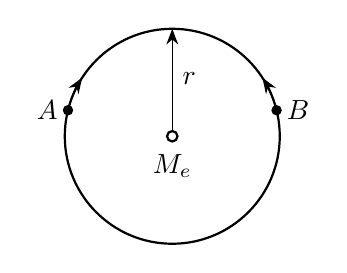
\begin{tikzpicture}[fig,scale=1.05]
 \draw (0,0) circle (1.3);
 \draw[->,line width=0.5pt] (0,0) -- (0,1.3); \node[right] at (0,0.7) {$r$};
 \draw[fill=white] (0,0) circle (1.8pt); \node[below] at (0,-0.1) {$M_e$};
 \fill (166:1.3) circle (1.8pt); \node[left] at (166:1.3) {$A$};
 \fill (14:1.3) circle (1.8pt); \node[right] at (14:1.3) {$B$};
 \draw[->,line width=0.5pt] (166:1.3) arc (166:147:1.3);
 \draw[->,line width=0.5pt] (14:1.3) arc (14:33:1.3);
\end{tikzpicture}}

% Motion Ex-III Q.15 : sphere with spherical hole
\newcommand{\figHole}{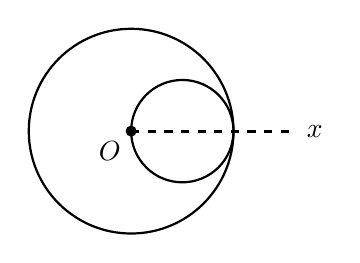
\begin{tikzpicture}[fig]
 \draw (0,0) circle (1.3); \draw (0.65,0) circle (0.65);
 \fill (0,0) circle (2pt); \node[below left] at (0,0) {$O$};
 \draw[dashed,line width=1pt] (0,0)--(2.1,0); \node[right] at (2.1,0) {$x$};
\end{tikzpicture}}

% Motion Ex-IV Q.3 : infinite rod with lambda(x) = lambda / x
\newcommand{\figInfRod}{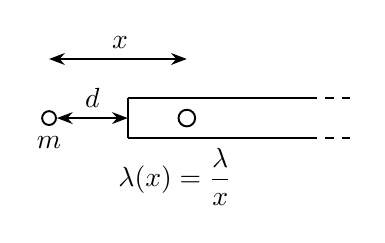
\begin{tikzpicture}[fig,line width=0.7pt]
 \draw (0,0) circle (2.5pt); \node[below] at (0,-0.1) {$m$};
 \draw[<->] (0.1,0)--(1.0,0); \node[above] at (0.55,0) {$d$};
 \draw (1.0,-0.25)--(1.0,0.25); \draw (1.0,0.25)--(3.3,0.25); \draw (1.0,-0.25)--(3.3,-0.25);
 \draw[dashed] (3.3,0.25)--(3.9,0.25); \draw[dashed] (3.3,-0.25)--(3.9,-0.25);
 \draw[fill=white] (1.75,0) circle (3pt);
 \draw[<->] (0,0.75)--(1.75,0.75); \node[above] at (0.9,0.75) {$x$};
 \node at (1.6,-0.75) {$\lambda(x)=\dfrac{\lambda}{x}$};
\end{tikzpicture}}

% Nucleus JM Q.10 (JEE Main 2017) : g versus d
\newcommand{\gpanel}[2]{\begin{tikzpicture}[fig,line width=0.7pt,scale=0.85]
 \draw[->] (0,0)--(2.4,0) node[right] {\scriptsize $d$}; \draw[->] (0,0)--(0,1.8) node[above] {\scriptsize $g$};
 \node[below left] at (0,0) {\scriptsize $O$}; \node[left] at (-0.25,0.9) {(#1)};
 #2
\end{tikzpicture}}
\newcommand{\figGraphs}{%
 \gpanel{1}{\draw (0,0) .. controls (0.9,0) and (1.5,0.3) .. (1.95,1.6);}\hspace{0.6cm}
 \gpanel{2}{\draw (0,0) .. controls (0.6,0.05) and (0.95,0.5) .. (1.1,1.5) .. controls (1.25,0.5) and (1.7,0.08) .. (2.2,0.02);
  \draw[dotted] (1.1,0)--(1.1,1.5); \node[below] at (1.1,0) {\scriptsize $R$};}\\[6pt]
 \gpanel{3}{\draw (0,0) .. controls (0.6,0.05) and (0.95,0.5) .. (1.1,1.5) -- (1.85,0);
  \draw[dotted] (1.1,0)--(1.1,1.5); \node[below] at (1.1,0) {\scriptsize $R$};}\hspace{0.6cm}
 \gpanel{4}{\draw (0,0)--(1.1,1.5) .. controls (1.25,0.5) and (1.7,0.08) .. (2.2,0.02);
  \draw[dotted] (1.1,0)--(1.1,1.5); \node[below] at (1.1,0) {\scriptsize $R$};}}

% Nucleus JM Q.8 (JEE Main 2015) : sphere with cavity
\newcommand{\figCavityHatch}{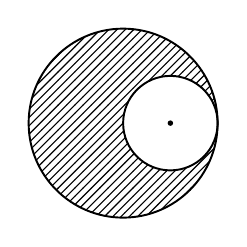
\begin{tikzpicture}[fig,line width=0.7pt]
 \path[pattern=north east lines,even odd rule] (0,0) circle (1.2) (0.6,0) circle (0.6);
 \draw (0,0) circle (1.2); \draw (0.6,0) circle (0.6); \fill (0.6,0) circle (1pt);
\end{tikzpicture}}

% Nucleus JM Q.35 (JEE Main 2021) : two satellites
\newcommand{\figTwoSat}{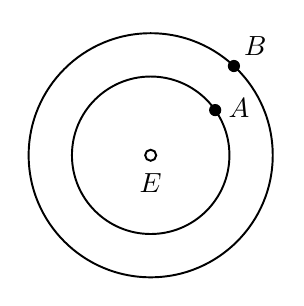
\begin{tikzpicture}[fig,line width=0.7pt]
 \draw (0,0) circle (1.0); \draw (0,0) circle (1.55);
 \draw[fill=white] (0,0) circle (2pt); \node[below] at (0,-0.1) {$E$};
 \fill (35:1.0) circle (2.2pt); \node[right] at (35:1.05) {$A$};
 \fill (47:1.55) circle (2.2pt); \node[above right] at (47:1.55) {$B$};
\end{tikzpicture}}

% JEE Main 2025 22 Jan Morning : sphere with spherical part removed
\newcommand{\figHoleP}{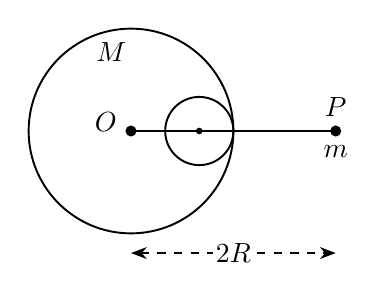
\begin{tikzpicture}[fig,line width=0.7pt]
 \draw (0,0) circle (1.3); \draw (0.867,0) circle (0.433);
 \fill (0,0) circle (2pt); \node[left] at (-0.05,0.12) {$O$};
 \fill (0.867,0) circle (1.2pt);
 \draw (0,0)--(2.6,0); \fill (2.6,0) circle (2pt);
 \node[above] at (2.6,0.05) {$P$}; \node[below] at (2.6,-0.05) {$m$};
 \node at (-0.25,1.0) {$M$};
 \draw[<->,dashed] (0,-1.55)--(2.6,-1.55); \node[fill=white,inner sep=1pt] at (1.3,-1.55) {$2R$};
\end{tikzpicture}}

% ---------- title block, answer key items, self assessment ----------
\newcommand{\titleblock}[2]{%
 \begin{center}
  {\Large\bfseries PRACTICE SHEET -- \sheetno}\\[2pt]
  {\normalsize\bfseries #1}
 \end{center}
 \vspace{1pt}
 \noindent\begin{tabularx}{\linewidth}{|X|X|X|}\hline
  Name: \hrulefill & Class / Section: \hrulefill & Date: \hrulefill \\ \hline
  \textbf{Time Allowed: 60 Mins} & \textbf{Total Questions: #2} & Roll No.: \hrulefill \\ \hline
 \end{tabularx}
 \par\vspace{4pt}}
\newcommand{\keyitem}[3]{\par\noindent\begin{minipage}{\linewidth}\textbf{#1.} {\scriptsize\color{spsgrey}[#2]}\ \ #3\end{minipage}\par\vspace{5pt}}

\newcommand{\selfassess}{%
 \clearpage
 \begin{center}{\Large\bfseries SELF ASSESSMENT -- Practice Sheet \sheetno}\end{center}
 \noindent\textit{Fill this in after checking your answers with the Answer Key.}\par\vspace{6pt}
 \noindent\begin{tabularx}{\linewidth}{|X|X|}\hline
  \textbf{Time Allowed:} 60 Mins & \textbf{Time Taken:} \rule{2.2cm}{0.4pt} Mins \\ \hline
  Start time: \rule{2cm}{0.4pt} & End time: \rule{2cm}{0.4pt} \\ \hline
  \multicolumn{2}{|l|}{Finished within the allowed time?\quad $\square$ Yes \quad $\square$ No \quad (extra / saved time: \rule{1.6cm}{0.4pt} Mins)} \\ \hline
 \end{tabularx}
 \par\vspace{8pt}
 \noindent\begin{tabularx}{\linewidth}{|>{\centering\arraybackslash}X|>{\centering\arraybackslash}X|>{\centering\arraybackslash}X|>{\centering\arraybackslash}X|>{\centering\arraybackslash}X|}\hline
  \textbf{Total} & \textbf{Attempted} & \textbf{Correct} & \textbf{Incorrect} & \textbf{Not attempted} \\ \hline
  15 & \rule[-4pt]{0pt}{18pt} & & & \\ \hline
 \end{tabularx}
 \par\vspace{3pt}
 \noindent Score (Correct $/$ 15): \rule{1.8cm}{0.4pt} \qquad Percentage: \rule{1.8cm}{0.4pt}\,\%
 \par\vspace{8pt}
 \noindent\textbf{Question-wise tracker} \hfill {\footnotesize write \ding{51} (correct), \ding{55} (incorrect) or $-$ (not attempted)}\par\vspace{3pt}
 \noindent\begin{tabularx}{\linewidth}{|*{8}{>{\centering\arraybackslash}X|}}\hline
  1&2&3&4&5&6&7&8\\ \hline \rule[-5pt]{0pt}{18pt}&&&&&&&\\ \hline
  9&10&11&12&13&14&15& \\ \hline \rule[-5pt]{0pt}{18pt}&&&&&&&\\ \hline
 \end{tabularx}
 \par\vspace{8pt}
 \noindent\textbf{Reason for the incorrect / unattempted questions} (write question numbers)\par\vspace{2pt}
 \noindent\begin{tabularx}{\linewidth}{|X|X|}\hline
  Concept not clear: \hrulefill & Formula forgotten: \hrulefill \\ \hline
  Calculation / silly mistake: \hrulefill & Ran out of time: \hrulefill \\ \hline
 \end{tabularx}
 \par\vspace{8pt}
 \noindent\textbf{Personal feedback guide (tick the band that matches your score)}\par\vspace{2pt}
 \noindent\begin{tabularx}{\linewidth}{|c|c|X|}\hline
  & \textbf{Correct} & \textbf{What to do next} \\ \hline
  $\square$ & 14--15 & Excellent. Concept and speed are both strong. Move to harder JEE-level problems and keep revising formulae once a week. \\ \hline
  $\square$ & 11--13 & Good. Re-do every incorrect question without looking at the solution, then note the formula or idea you missed. \\ \hline
  $\square$ & 7--10 & Fair. Revise the theory of escape speed, orbital speed, energies of a satellite and Kepler's laws, then re-attempt this sheet after 3 days. \\ \hline
  $\square$ & 0--6 & Needs attention. Re-read the chapter notes and solved examples first, then attempt this sheet again in two parts of 30 mins. \\ \hline
 \end{tabularx}
 \par\vspace{8pt}
 \noindent\textbf{My personal feedback / action plan:}\par\vspace{4pt}
 \noindent\rule{\linewidth}{0.4pt}\par\vspace{9pt}\noindent\rule{\linewidth}{0.4pt}\par\vspace{9pt}\noindent\rule{\linewidth}{0.4pt}\par\vspace{9pt}\noindent\rule{\linewidth}{0.4pt}
 \par\vspace{10pt}
 \noindent\textbf{Teacher's remarks:}\par\vspace{4pt}
 \noindent\rule{\linewidth}{0.4pt}\par\vspace{9pt}\noindent\rule{\linewidth}{0.4pt}
 \par\vspace{14pt}
 \noindent Student's signature: \rule{4cm}{0.4pt} \hfill Teacher's signature: \rule{4cm}{0.4pt}}
\newcommand{\sheetno}{1}
\newcommand{\sheettopic}{Gravitation -- Level 1 (Foundation)}
\begin{document}
\titleblock{Gravitation -- Level 1 (Foundation): Practice Sheet 1 of 3}{15}
\noindent\textbf{Instructions:} Attempt all 15 questions; each has only one correct option. Sections: A -- Acceleration due to Gravity, B -- Gravitational Potential and Potential Energy, C -- Motion of Satellite, D -- Newton's Law, Gravitational Field and Kepler's Laws. Time Allowed: 60 Mins.

\begin{multicols}{2}
\letterlabels
\secthead{Section A -- Acceleration due to Gravity}

\begin{question}{Motion, Ex-I Q.1}
At what altitude will the acceleration due to gravity be 25\% of that at the earth's surface (given radius of earth is $R$)?
\optstwo{$R/4$}{$R$}{$3R/8$}{$R/2$}
\end{question}

\begin{question}{JEE Main 2024, 6th April Evening Shift}
Assuming the earth to be a sphere of uniform mass density, a body weighed 300 N on the surface of earth. How much it would weigh at $R/4$ depth under surface of earth?
\optstwo{75 N}{375 N}{300 N}{225 N}
\end{question}

\begin{question}{JEE Main 2024, 4th April Evening Shift}
A 90 kg body placed at $2R$ distance from surface of earth experiences gravitational pull of: ($R$ = Radius of earth, $g=10$ m s$^{-2}$)
\optstwo{300 N}{225 N}{100 N}{120 N}
\end{question}

\begin{question}{Motion, Ex-I Q.4}
If the radius of the earth be increased by a factor of 5, by what factor its density be changed to keep the value of $g$ the same?
\optstwo{$1/25$}{$1/5$}{$1/\sqrt5$}{$5$}
\end{question}

\secthead{Section B -- Gravitational Potential and Potential Energy}

\begin{question}{JEE Main 2024, 6th April Morning Shift}
To project a body of mass $m$ from earth's surface to infinity, the required kinetic energy is (assume, the radius of earth is $R_E$, $g=$ acceleration due to gravity on the surface of earth):
\optstwo{$\frac12 mgR_E$}{$4mgR_E$}{$mgR_E$}{$2mgR_E$}
\end{question}

\begin{question}{Motion, Ex-I Q.11}
A hollow spherical shell is compressed to half its radius. The gravitational potential at the centre
\optstwo{increases}{decreases}{remains same}{during the compression increases then returns at the previous value}
\end{question}

\begin{question}{JEE Main 2025, 28th January Evening Shift}
Earth has mass 8 times and radius 2 times that of a planet. If the escape velocity from the earth is 11.2 km/s, the escape velocity in km/s from the planet will be:
\optstwo{8.4}{11.2}{5.6}{2.8}
\end{question}

\begin{question}{Motion, Ex-I Q.10}
The escape velocity for a planet is $v_e$. A tunnel is dug along a diameter of the planet and a small body is dropped into it at the surface. When the body reaches the centre of the planet, its speed will be
\optsfour{$v_e$}{$\dfrac{v_e}{\sqrt2}$}{$\dfrac{v_e}{2}$}{zero}
\end{question}

\secthead{Section C -- Motion of Satellite}

\begin{question}{Motion, Ex-I Q.17}
A satellite of the earth is revolving in circular orbit with a uniform velocity $V$. If the gravitational force suddenly disappears, the satellite will
\optsone{continue to move with the same velocity in the same orbit}
{move tangentially to the original orbit with velocity $V$}
{fall down with increasing velocity}
{come to a stop somewhere in its original orbit}
\end{question}

\begin{question}{Motion, Ex-I Q.18}
A satellite revolves in the geostationary orbit but in a direction east to west. The time interval between its successive passing about a point on the equator is
\optstwo{48 hrs}{24 hrs}{12 hrs}{never}
\end{question}

\begin{question}{JEE Main 2025, 23rd January Evening Shift}
If a satellite orbiting the Earth is 9 times closer to the Earth than the Moon, what is the time period of rotation of the satellite? Given rotational time period of Moon $=27$ days and gravitational attraction between the satellite and the moon is neglected.
\optstwo{3 days}{27 days}{81 days}{1 day}
\end{question}

\secthead{Section D -- Newton's Law, Gravitational Field and Kepler's Laws}

\begin{question}{Motion, Ex-I Q.16}
A mass is at the center of a square, with four masses at the corners as shown.
\begin{center}\figSquares\end{center}
Rank the choices according to the magnitude of the gravitational force on the center mass.
\optstwo{$F_A=F_B<F_C=F_D$}{$F_A>F_B<F_D<F_C$}{$F_A=F_B>F_C=F_D$}{none}
\end{question}

\begin{question}{Motion, Ex-I Q.26}
A planet of mass $m$ is in an elliptical orbit about the sun ($m\ll M_{sun}$) with an orbital period $T$. If $A$ be the area of orbit, then its angular momentum would be
\optstwo{$\dfrac{2mA}{T}$}{$mAT$}{$\dfrac{mA}{2T}$}{$2mAT$}
\end{question}

\begin{question}{JEE Main 2026, 2nd April Morning Shift}
A planet ($P_1$) is moving around the star of mass $2M$ in the orbit of radius $R$. Another planet ($P_2$) is moving around another star of mass $4M$ in a orbit of radius $2R$. Ratio of time periods of revolution of $P_2$ and $P_1$ is \underline{\hspace{1cm}}.
\optstwo{$\dfrac12$}{$2$}{$4$}{$\dfrac14$}
\end{question}

\begin{question}{JEE Main 2024, 1st February Evening Shift}
A light planet is revolving around a massive star in a circular orbit of radius $R$ with a period of revolution $T$. If the force of attraction between planet and star is proportional to $R^{-3/2}$ then choose the correct option:
\optstwo{$T^2\propto R^{7/2}$}{$T^2\propto R^{3}$}{$T^2\propto R^{5/2}$}{$T^2\propto R^{3/2}$}
\end{question}
\end{multicols}

%==================== ANSWER KEY ====================
\clearpage
\begin{center}{\Large\bfseries ANSWER KEY -- Practice Sheet \sheetno}\end{center}
\noindent{\small Answers are taken from the source answer keys: Motion (Answer Ex-I) and the JEE PYQ file (Answer Key at the end).}\par\vspace{4pt}
\begin{multicols}{2}
\keyitem{1}{Motion Ex-I Q.1}{B}
\keyitem{2}{JEE PYQ file Q.22}{D}
\keyitem{3}{JEE PYQ file Q.26}{C}
\keyitem{4}{Motion Ex-I Q.4}{B}
\keyitem{5}{JEE PYQ file Q.23}{C}
\keyitem{6}{Motion Ex-I Q.11}{B}
\keyitem{7}{JEE PYQ file Q.14}{C}
\keyitem{8}{Motion Ex-I Q.10}{B}
\keyitem{9}{Motion Ex-I Q.17}{B}
\keyitem{10}{Motion Ex-I Q.18}{C}
\keyitem{11}{JEE PYQ file Q.16}{D}
\keyitem{12}{Motion Ex-I Q.16}{A}
\keyitem{13}{Motion Ex-I Q.26}{A}
\keyitem{14}{JEE PYQ file Q.5}{B}
\keyitem{15}{JEE PYQ file Q.29}{C}
\end{multicols}

\selfassess
\end{document}
